% ~~~~~~~~~~~~~~~~~~~~~~~~~~~~~~~~~~~~~~~~~~~~~~~~~~~~~~~~~~~~~~~~~~~~~~~~~~~~~
%                                 IMPLEMENTATION
% ~~~~~~~~~~~~~~~~~~~~~~~~~~~~~~~~~~~~~~~~~~~~~~~~~~~~~~~~~~~~~~~~~~~~~~~~~~~~~
\chapter{Implementation}\label{chap:4}
  \lhead{Chapter 4. \emph{Implementation}}

\section{Game}
Game class is often implemented as a set of tools operating on provided state.
With this approach, tests can be easily designed to verify functionality.
In many cases, following methods or attributes are available:
\begin{itemize}
  \vspace*{-0.25cm}
  \setlength\itemsep{-0.15cm}

  \item initial\_state - initial state of the game
  \item is\_terminal - whether the given state is terminal
  \item valid - validates given state or action on the given state
  \item actions - list of all possible actions in the given state
  \item execute\_move - returns new state after executing given action
  \item utility - value representing how the given state is beneficial
                  for given player

  \vspace*{-0.25cm}
\end{itemize}

\noindent I consider following methods also important in Quoridor, so these are
present in my implementation:
\begin{itemize}
  \vspace*{-0.25cm}
  \setlength\itemsep{-0.15cm}

  \item undo - previous state before provided action and state
  \item shortest\_path - shortest path to goal row for the given player
  \item path\_blockers - set of wall positions that could block the given path
  \item crossing\_actions - set of invalid actions that would cross already
                            placed walls

  \vspace*{-0.25cm}
\end{itemize}

\section{State}
State should be the smallest possible representation of the game state where
it can be easily distinguished between any two different states. Mathematicaly,
state $S$ can be defined as:
\begin{equation}
  \label{eqn:state_def}
  S = (c, p_y, p_g, s_y, s_g, w)
  \vspace*{-0.20cm}
\end{equation}
Here, $c\in\{0, 1\} $ represents color of the player that should move,
$p_y,p_g\in\{0,1,...,80\}$ are pawns positions,
${s_y},{s_g} \in \{0, 1, ..., 10\}$ are counts of walls in stocks,
and set of positions of placed walls are
${w = \{\,a_i\,|\,a_i \in \{0, 1, ..., 127\}, i \in \{0, 1, ..., 20\} \}}$.
One such state in python would be:
\begin{lstlisting}
state = (0, 51, 70, 5, 9, frozenset([32, 116, 119, 59, 12, 31]))
\end{lstlisting}

However, when training ANN, it may be better to convert it to zeroes and ones.
TODO


\section{Context}
For speeding up validation of the moves for agents, it turned out to be faster
to keep in memory shortest paths and invalid actions such as crossing walls.
Also, this speeded up the decision process of heuristic and path agents.

\section{Console Game}
\begin{wrapfigure}{r}{0.5\textwidth}
  \vspace*{-2.05cm}
  \centering
  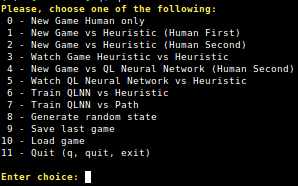
\includegraphics[width=0.48\textwidth]{main_menu.png}
  \vspace*{-0.35cm}
  \caption{main menu}
  \label{fig:main_menu}
  \vspace*{-0.70cm}
\end{wrapfigure}

Main purpose of my work was on implementation of the agent utilizing abilities
of the ANN, so the game is played and displayed in the linux terminal
(console), and so, all interactions are performed through command prompt.
To display the game properly in the terminal, it must be at least 86 characters
wide.

In the main menu (fig. \ref{fig:main_menu}), user can choose to play a game
against HeuristicPlayer (HP) or QLNNPlayer (QLNN) and also, watch game played
eighter by HP versus himself or against QLNN. Also, loading and saving a game
is possible.

\begin{wrapfigure}{l}{0.5\textwidth}
  \vspace*{-0.35cm}
  \centering
  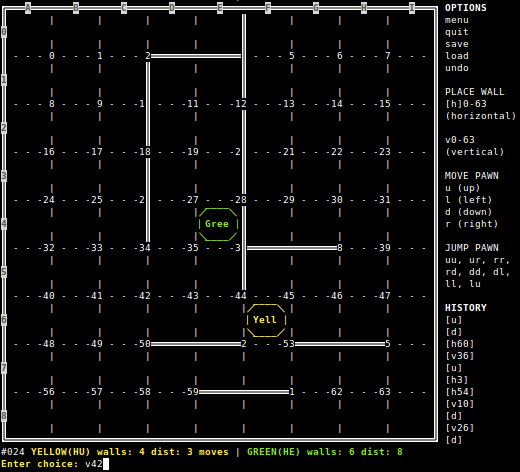
\includegraphics[width=0.49\textwidth]{game_running.png}
  \vspace*{-0.30cm}
  \caption{game running}
  \label{fig:game_running}
  \vspace*{-0.60cm}
\end{wrapfigure}

During the game (fig. \ref{fig:game_running}), human players enters to move his
pawn with first letters of words \textit{up, left, right, down}
(\textit{u, l, r, d}) and jumps over opponents pawn with combinations of simple
moves (\textit{uu, ul, ur, dd, dl, dr}). To specify wall placement, first
letters of direction are provided (\textit{h, v}) followed by number
of the position.  For example, \textit{h3}, \textit{v24} are correctly entered
wall positions. Other options available are \textit{undo, load} or
\textit{save}. On the right side along the options possible, user can see some
of the last moves in the HISTORY section. Below the board, there are displayed
move number, wall stocks, who moves and current distances from the goal.


% \begin{itemize}
%   \vspace*{-0.25cm}
%   \setlength\itemsep{-0.15cm}
% 
%   \item 
%   \item 
% 
%   \vspace*{-0.25cm}
% \end{itemize}

% \begin{itemize}
%   \vspace*{-0.25cm}
%   \setlength\itemsep{-0.15cm}
% 
%     \item 0 - New Game Human only
%     \item 1 - New Game vs Heuristic (Human First)
%     \item 2 - New Game vs Heuristic (Human Second)
%     \item 3 - Watch Game Heuristic vs Heuristic
%     \item 4 - New Game vs QL Neural Network (Human Second)
%     % \item 5 - Watch QL Neural Network vs Heuristic
%     % \item 6 - Train QLNN vs Heuristic
%     % \item 7 - Train QLNN vs Path
%     % TODO: rules
%     \item 8 - Generate random state
%     \item 9 - Save last game
%     \item 10 - Load game
%     \item 11 - Quit (q, quit, exit)
% 
%   \vspace*{-0.25cm}
% \end{itemize}

% \subsection{Game Menu}

\section{PathPlayer}
PathPlayer is an agent that only follows shortest path to the goal row. I have
used this agent as a reference to compare number of won games against
HeuristicPlayer and QlearningNetworkPlayer.

\section{HeuristicPlayer}
HeuristicPlayer's algorithm is following:
\begin{itemize}
  \vspace*{-0.25cm}
  \setlength\itemsep{-0.15cm}

  \item if no walls in stock, follow the shortest path
  \item if one step left to goal row, move to win
  \item if standing on the starting line, follow the shortest path
  \item if there are more than 2 possibilities to block (prolong) opponents
        path then with $60\%$ probability follow the shortest path
  \item if there are wall positions blocking opponent's path and not
        blocking it's own path and it would not cut opponent from goal row,
        place one such wall
  \item in all other cases, follow the shortest path

  \vspace*{-0.25cm}
\end{itemize}

\section{QLNNPlayer Training}
How I trained...TODO

\section{QLNNPlayer}
QLNNPlayer evaluates every action in the current state, takes action
with maximum value and tries to play it. If move is not possible, it tries to
play next best action.
